
\section{Węzły satelitarne}

% DIKTJONARY;latitude;szerokość geograficzna;geografia
% DIKTJONARY;longitude;długość geograficzna;geografia
% DIKTJONARY;meridian (of longitude);południk;geografia
% DIKTJONARY;parallel (of latitude);równoleżnik;geografia
% DIKTJONARY;---;geografia;-
% to jest powtórzenie np. z pliku 103a
Załóżmy, że w dopełnieniu pewnego splotu został zanurzony torus.
Jeżeli jest ściśliwy, to albo równoleżnikl torusa ogranicza dysk w dopełnieniu splotu~i torus jest niezawęźlony, albo południk ogranicza dysk w dopełnieniu splotu i~splot nie przebiega wzdłuż torusa.
Żadna z~tych sytuacji nie jest ciekawa.
Inny zdegenerowany przypadek występuje, gdy torus stanowi rurowe otoczenie jednego z~ogniw splotu.
W przeciwnym razie splot można zbudować z~prostszych obiektów.

Oto formalny opis konstrukcji.
Niech $W$ będzie pełnym torusem.
Dysk zanurzony w $W$, którego brzeg stanowi nieściągalną pętlę w $\partial W$, nazywamy południkowym.
Mówimy, że zamknięta krzywa $\lambda \subseteq W$ jest właściwa, jeżeli przecina wszystkie dyski południkowe.

\begin{definition}[węzeł satelitarny]
\index{węzeł!satelitarny}%
\index{wzorzec}%
\index{satelita}%
\index{towarzysz}%
    Niech $P$ będzie splotem zanurzonym w~torusie niezawęźlonym $W$ tak, by co najmniej jedno z~ogniw stanowiło właściwą pętlę w~$W$.
    Niech $C$ będzie węzłem, zaś $V$ jego rurowym otoczeniem.
    Wybierzmy dowolny homeomorfizm $h \colon W \to V$.
    Wtedy splot $S = h(P)$ nazywamy satelitą o~wzorcu $P$ i towarzyszu $C$.
\end{definition}

% \begin{definition}
%     Węzeł nazywamy satelitarnym, jeśli zawiera nieściśliwy, nierównoległy do brzegu torus we własnym dopełnieniu.
% \end{definition}

Taką definicję podają Burde, Zieschang, Heusener \cite[s. 21]{burde2014} (i wspominają, że towarzysze po niemiecku to Begleitknoten)

Hoste i inni \cite{thistlethwaite1998} podejrzewają, że jeśli satelita owija się $m$-krotnie wokół torusa, zaś indeks skrzyżowaniowy towarzysza wynosi $k$, to satelita nie posiada diagramu o~mniej niż $km^2$ skrzyżowaniach.
\index[persons]{Hoste, Jim}%
\index[persons]{Thistlethwaite, Morwen}%
\index[persons]{Weeks, Jeff}%

Ponieważ dla trójlistnika $k = 3$, napotkali się tylko na satelity owijające się $m = 2$ razy podczas tablicowania pierwszych węzłów do 16 skrzyżowań.
Nie spodziewano się żadnego satelity ósemki, gdyż wtedy $k = 4$, zatem każdy satelita miałby co najmniej $4 \cdot 2^2 + 1 = 17$ skrzyżowań: dodatkowe $+1$ jest potrzebne, by nie dostać splotu o~dwóch ogniwach.

Najprostszy satelita ma 13 skrzyżowań.
Ze strony internetowej programu Regina można dowiedzieć się dokładniej, jak wygląda rozkład satelitów wśród małych węzłów:

\renewcommand*{\arraystretch}{1.4}
\footnotesize
\begin{longtable}{lccccccc}
    \hline
    \textbf{skrzyżowania} & 13 & 14 & 15 & 16 & 17 & 18 & 19 \\ \hline \endhead
    węzły pierwsze, satelitarne & 2 & 2 & 6 & 10 & 29 & 86 & 245 \\
    \hline
\end{longtable}
\normalsize

Razem 380 węzłów.

\begin{example}[torus połykająco-podążający]
\label{swallow_follow_torus}
\index{torus połykająco-podążający}%
% DICTIONARY;swallow-follow;połykająco-podążający;torus
% DICTIONARY;torus;torus;-
    \begin{figure}[H]
        \centering
        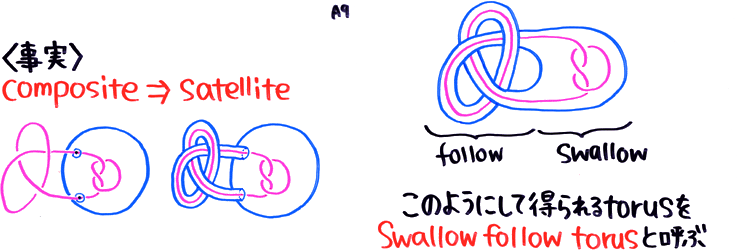
\includegraphics[width=0.75\linewidth]{../data/mixed/follow-swallow.png}
        \caption[something]{Torus połykająco-podążający. Źródło: strona internetowa  C. Hayashiego.}
    \end{figure}
    Klasa węzłów satelitarnych obejmuje węzły złożone.
    W ich przypadku można wskazać pewien szczególny torus nieściśliwy -- połykający pierwszy składnik, a~potem podążający za drugim\footnote{Źródło obrazka: \url{https://mcm-www.jwu.ac.jp/~hayashic/semi/07/07i/07i.html}}.
\end{example}

Schubert pokazał, że zorientowane klasy izotopii węzłów w~$S^3$ tworzą wolny przemienny monoid na przeliczalnie wielu generatorach.
\index[persons]{Schubert, Horst}%
Dowód to uważna analiza nieściśliwych torusów obecnych w~dopełnieniu sumy spójnej.
To doprowadziło go do definicji węzłów satelitarnych i~towarzyszących w~przełomowej pracy \cite{schubert1953} oraz zunifikowało teorię 3-rozmaitości z teorią węzłów.
Może warto zapoznać się z pracą Motegiego \cite{motegi1997}?
Wikipedia mówi, że zapis węzła jako satelity nie jest jednoznaczny, a~tam mogą być przykłady.
%=% https://en.wikipedia.org/wiki/Satellite_knot#cite_ref-7

Na brzegu torusa $V$ można wprowadzić pewien układ współrzędnych: południk to pętla właściwa w $\partial V$, która ogranicza dysk w $V$, natomiast równoleżnik to pętla w $\partial V$, która spotyka południk raz.
Z~dokładnością do izotopii południk jest jeden, ale równoleżnik nie.
Równoleżnik preferowany to taki, którego indeks zaczepienia z~rdzeniem torusa wynosi zero.

\begin{definition}[dubel Whiteheada]
\index{dubel Whiteheada}%
    Niech $P \subseteq W$ będzie jednokrotnie skręconym niewęzłem, tak jak na rysunku 3.1.2a w \cite[s. 32]{kawauchi1996}.
    Wtedy węzeł $S$ nazywamy dublem Whiteheada.
\end{definition}

Każdy węzeł posiada nieskończenie wiele dubli Whiteheada: wystarczy rozciąć torus $V$, skręcić jedną końcówkę i~ponownie zszyć, żaden z~nich nie jest odróżniany od niewęzła przez wielomian Alexandera.

Wyróżnia się pewien szczególny homeomorfizm $h$, który przenosi południk i preferowany równoleżnik $W$ na południk i preferowany równoleżnik $V$.
Nazywamy go wiernym.
% DICTIONARY;faithful homeomorphism;homomorfizm wierny;-
O dublu względem wiernego homeomorfizmu mówimy, że jest nieskręcony.
% TODO: skąd powyższe zdanie -- z Kawauchi około strony 32 (Ten z 1996)
% TODO: Usually, we take the homeomorphism cp to send the the standard meridian-longitude system (Co, mo) of V to a meridian-longitude system (C, m) of K on V*, which we call a faithful homeomorphism.

\begin{definition}[węzeł kablowy]
\index{węzeł!kablowy}%
    Niech $h \colon W \to V$ będzie wiernym homeomorfizmem, zaś $P$ węzłem $(p, q)$-torusowym.
    Satelitę $S$ nazywamy węzłem $(p, q)$-kablowym albo krótko kablem.
\end{definition}

\begin{proposition}
    Każdy kabel wyznacza jednoznacznie węzeł, z~którego powstał.
\end{proposition}

\begin{proof}
\index[persons]{Feustel, Charles}%
\index[persons]{Whitten, Wilbur}%
    Wniosek 2 z~pracy Feustela, Whittena \cite{feustel1978} pokazuje, że na podstawie kabla można wyznaczyć parametry węzła torusowego $K'_{p,q}$ oraz topologię dopełnienia oryginalnego węzła.
    Ale my wiemy już dzięki z~twierdzenia Gordona-Lueckego, że różne węzły pierwsze mają różne dopełnienia... co jakoś kończy dowód.
\end{proof}

Niewęzeł nie ma nietrywialnych towarzyszy (węzłów towarzyszących).

\begin{definition}
\index{towarzysz!właściwy}%
    Towarzysza $C$ nietrywialnego splotu nazywamy właściwym, jeśli nie jest niewęzłem i~nie jest ogniwem tego splotu.
\end{definition}

Sploty bez właściwych towarzyszy określa się zazwyczaj terminem ,,atoroidalny''.
\index{splot!atoroidalny}%
Patrz też diagram przedstawiony u Cromwella \cite[s. 83]{cromwell2004}.

Schubert \cite{schubert1954} zastanawiał się, czy węzeł może mieć nieskończenie wiele towarzyszy.
\index[persons]{Schubert, Horst}%
Udzielił negatywnej odpowiedzi: satelita $S$ z towarzyszem $C$ oraz wzorcem indeksu $k$ spełnia nierówność $\bridge(S) \ge k \cdot \bridge(C)$; z drugiej strony tylko niewęzeł jest 1-mostowy.
(Patrz też wstęp do artykułu Schultens \cite{schultens2003}, skąd dowiedzieliśmy się o tych ciekawostkach).
(Trochę dużo tych ,,patrz też'').
% wiem to z pracy schultens03

\begin{proposition}
\index{węzeł!kablowy}%
\index{dubel Whiteheada}%
    Duble nietrywialnych węzłów oraz kable są pierwsze.
\end{proposition}

\begin{proof}
    Prosty wniosek z~twierdzenia 4.4.1 Cromwella \cite[s. 84]{cromwell2004}: jeżeli wzorzec jest niewęzłem lub węzłem pierwszym, to każdy właściwy satelita jest pierwszy.
\end{proof}

Niektóre węzły przedstawiają się jako satelity w~dokładnie jeden sposób, inne nie.
Rok 1979 przyniósł amerykańską pracę \cite{jaco1979} oraz niemiecką książkę\footnote{Według recenzji Hempela, najważniejsze tam jest twierdzenie klasyfikacyjne: niech $M_1, M_2$ będą 3-rozmaitościami Hakena \index{rozmaitość!Hakena} z brzegiem, zaś $V_1, V_2$ ich podrozmaitościami charakterystycznymi, wtedy każdą homotopijną równoważność $f \colon M_1 \to M_2$ można zdeformować tak, że jest homeomorfizmem między domknięciami: $M_1 \setminus V_1$ oraz $M_2 \setminus V_2$ i~homotopijną równoważnością między $V_1$ oraz $V_2$.} \cite{johannson1979}, gdzie niezależnie od siebie opisano jednoznaczny rozkład (nazywany teraz) Jaco-Shalena-Johannsona:
\index{rozkład Jaco-Shalena-Johannsona}%
\index[persons]{Jaco, William}%
\index[persons]{Shalen, Peter}%
\index[persons]{Johannson, Klaus}%

\begin{proposition}
    Niech $M$ będzie nierozkładalną, orientowalną, domkniętą 3-rozmaitością.
    Wtedy istnieje minimalna rodzina rozłącznie zanurzonych nieściśliwych torusów tak, że każda składowa 3-rozmaitości powstałej przez rozcinanie wzdłuż torusów jest:
    \begin{itemize}
        \item atoroidalna lub
    \item włóknistą przestrzenią Seiferta ($S^1$-wiązką nad dwuwymiarowym orbifoldem).    \end{itemize}
\index{orbifold}%
\index{rozmaitość!atoroidalna}%
\index{przestrzeń!włóknista Seiferta}%
\index{wiązka ($S^1$)}%
\index{torus nieściśliwy}%
    Rodzina ta z dokładnością do izotopii jest jedyna.
\end{proposition}

Jest on związany z operacją złączania (ang. \emph{splicing}), będącej uogólnieniem budowania satelitów, sumy spójnej, dubli Whiteheada i kasowania ogniwa.
\index{złączanie (splicing)}%
% https://arxiv.org/pdf/math/0506523.pdf
% DICTIONARY;splicing;złączanie;-
Hipotezę o jedyności rozkładu wysnuł wcześniej Waldhausen.
\index[persons]{Waldhausen, Friedhelm}%

% Koniec sekcji Węzły satelitarne

